% flashcards-title: Number line from 0 to 10 with two labeled dots
% flashcards-desc: A horizontal number line with evenly spaced marks labeled 0 through 10 and an arrowhead pointing right beyond 10. A round dot labeled A sits on the mark at 3, and a round dot labeled B sits on the mark at 8.
\documentclass[tikz]{standalone}
\usetikzlibrary{arrows.meta,patterns}

\definecolor{qraNavy}{HTML}{17324D}
\definecolor{qraBlue}{HTML}{2B6CB0}
\definecolor{qraGold}{HTML}{B7791F}
\definecolor{qraPale}{HTML}{EAF2F8}
\definecolor{qraGray}{HTML}{5C6773}

\tikzset{
  qra axis/.style={draw=qraNavy, line width=1.2pt},
  qra tick/.style={draw=qraNavy, line width=1pt},
  qra guide/.style={draw=qraGray, densely dashed, line width=0.8pt},
  qra counter/.style={circle, draw=qraNavy, fill=qraPale, line width=0.9pt, minimum size=7mm, inner sep=0pt},
  qra label/.style={font=\sffamily\bfseries, text=qraNavy},
  qra small label/.style={font=\sffamily, text=qraNavy},
}

\begin{document}
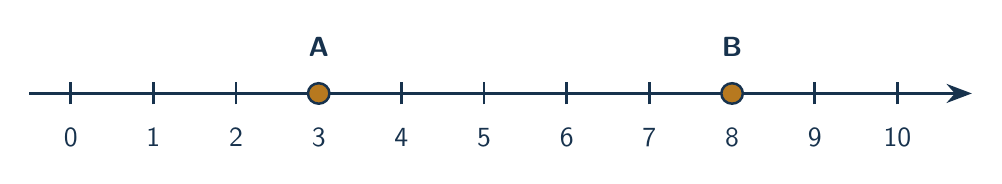
\begin{tikzpicture}[x=1.05cm]
  % Axis with rightward arrow to show the line continues
  \draw[qra axis, -{Stealth[length=3.2mm]}] (-0.5,0) -- (10.9,0);

  % Ticks and labels 0..10
  \foreach \n in {0,...,10} {
    \draw[qra tick] (\n,-0.14) -- (\n,0.14);
    \node[qra small label, below=2mm] at (\n,-0.12) {\n};
  }

  % Dot A on 3 and dot B on 8, with letter labels above
  \filldraw[fill=qraGold, draw=qraNavy, line width=0.9pt] (3,0) circle (0.13);
  \node[qra label, above=2.5mm] at (3,0.1) {A};
  \filldraw[fill=qraGold, draw=qraNavy, line width=0.9pt] (8,0) circle (0.13);
  \node[qra label, above=2.5mm] at (8,0.1) {B};
\end{tikzpicture}
\end{document}
